\section{Regularization}
\label{sec:ch4:regularization}

In practice, many networks you will encounter in network machine learning will \emph{not} be simple networks. As we discussed in the preceding discussion, many of the techniques we discuss will be just fine to use with weighted networks. Unfortunately, real world networks are often extremely noisy, and so the analysis of one real world network might not generalize very well to a similar real world network. For this reason, we turn to \emph{regularization}. 

\textit{Regularization} is the process by which you either:
\begin{enumerate}
    \item Modify data for the purpose of mitigating overfitting due to idiosyncrasies of the observed data, and/or
    \item Modify the function you are estimating due to its fragility to the idiosyncracies of the observed data.
\end{enumerate}

In network machine learning, the first step of your analysis is to typically modify the network (or networks) themselves to allow better generalization of your statistical inference to new datasets. Later chapters, such as Section \ref{sec:ch6} and many areas of the Applications, will cover approaches in which you modify the function you are estimating.

For each of the following subsections, we'll pose an example, a simulation, and code for how to implement the desired regularization approach. It is important to realize that you might use several of these techniques simultaneously in practice, or you might have a reason to use these techniques that go outside of our working examples.

To start this section off, we're going a few running examples for this section. We have two non-simple networks:

\begin{floatingbox}[h]\caption{Activity/hobby network}
The nodes of this network are a group of $50$ area students, the first $25$ of whom are athletes, and the second $25$ are in marching band. To collect the first network, you ask each student to select from a list of $50$ school activities and outside hobbies that they enjoy. For a pair of students $i$ and $j$, the weight of their interest alignment will be a score between $0$ and $50$ indicating how many activities or hobbies that they have in common. 

We will refer to this network as the activity/hobby network. This network is obviously undirected, since if student $i$ shares $x$ activities or hobbies with student $j$, then student $j$ also shares $x$ activities or hobbies with student $i$. This network is weighted, since the score is between $0$ and $50$. Finally, this network is loopless, because it would not make sense to look at the activity/hobby alignment of a student with themself, since this number would be largely uninformative as every student would have perfect alignment of activities and hobbies with him or herself. 

Because the network is undirected, the researchers have only saved half the portion of the adjacency matrix that includes the entries $a_{ij}$ where $j > i$. You will learn a strategy later to recover the full adjacency matrix.
\end{floatingbox}

\begin{floatingbox}[h]\caption{Friendship network}
This network is collected using the same $50$ students as the activity/hobby network. To collect the second network, you ask each student to rate how good of friends they are with other students, on a scale from $0$ to $1$. A score of $0$ means they are not friends with the student or do not know the student, and a score of $1$ means the student is their best friend. We will refer to this network as the friendship network. This network is clearly directed, since two students may differ on their understanding of how good of friends they are. This network is weighted, since the score is between $0$ and $1$. Finally, this network is also loopless, because it would not make sense to ask somebody how good of friends they are with themself.
\end{floatingbox}

Our scientific question of interest is how well activities and hobbies align with perceived notions of friendship. You want to use the preceding networks to learn about a hypothetical third network, a network whose nodes are identical to the two networks above, but whose edges are whether the two individuals are friends (or not) on facebook. To answer this question, you have quite the job to do to make your networks better suited to the task! We'll begin by simulating some example networks, which you can see in Figure \ref{fig:ch4:friendex}.

\begin{lstlisting}[style=python]
from graspologic.simulations import sbm
import numpy as np

wtargsa = [[dict(n=50, p=.09), dict(n=50, p=.02)],
          [dict(n=50, p=.02), dict(n=50, p=.06)]]

wtargsf = [[dict(a=4, b=2), dict(a=2, b=5)],
          [dict(a=2, b=5), dict(a=6, b=2)]]

# activity network as upper triangle matrix
A_activity_uppertri = sbm(n=[25, 25], p=[[1,1], [1,1]], wt=np.random.binomial, wtargs=wtargsa, loops=False, directed=False)
A_activity_uppertri = np.triu(A_activity_uppertri)

# friend network
A_friend = sbm(n=[25, 25], p=[[.8, .4], [.4, 1]], wt=np.random.beta, wtargs=wtargsf, directed=True)
\end{lstlisting}

\begin{figure}[h]
    \centering
    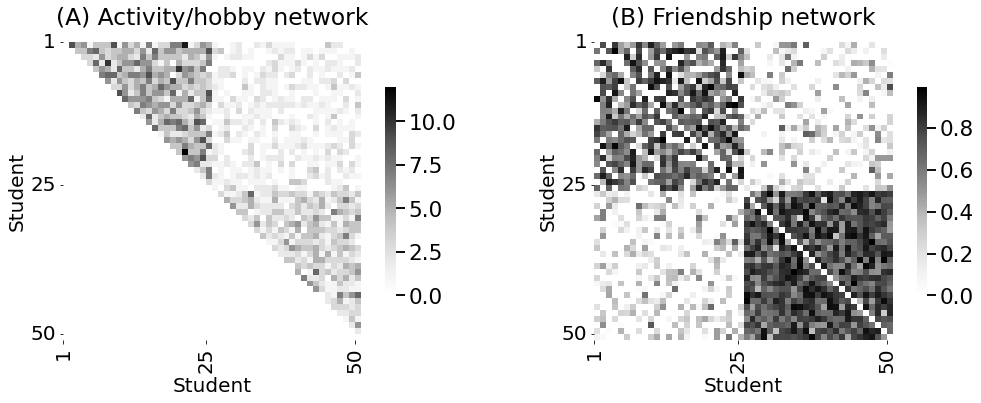
\includegraphics[width=\linewidth]{representations/ch4/Images/friendex.png}
    \caption[Friendship and activities networks]{A comparison of the two networks that we sampled to use in this section. The friendship network is shown in \textbf{(A)}, and the activity/hobby network is shown in \textbf{(B)}.}
    \label{fig:ch4:friendex}
\end{figure}

For good measure, we'll also work with a third network which will have unique particularities from the preceding two, where we want to ask a question about only this network itself. 
\begin{floatingbox}[h]\caption{Unrelated business network}
The $17$ nodes in the network are local businesses, and an edge exists between a pair of businesses if they have business dealings with one another (they buy or sell products from/with the company). Three of these businesses operate in total exclusion and do not have any edges. Three of these businesses only work with one other business. One businesses work with all of the non-excluded businesses. 
\end{floatingbox}

To begin, we're going to start looking at the business network. Let's take a look at what this network looks like in Figure \ref{fig:ch4:businessex}.

\begin{lstlisting}[style=python]
from graphbook_code import heatmap
from matplotlib import pyplot as plt
from graspologic.simulations import er_np
import networkx as nx

n = 10
A_bus = er_np(n, 0.6)

# add pendants
n_pend = 3
A_bus = np.column_stack([np.row_stack([A_bus, np.zeros((n_pend, n))]), 
                         np.zeros((n + n_pend, n_pend))])

n = n + n_pend
# add pizza hut node
n_pizza = 1
A_bus = np.column_stack([np.row_stack([A_bus, np.ones((n_pizza, n))]), 
                         np.ones((n + n_pizza, n_pizza))])
n = n + n_pizza

# add isolates
n_iso = 3
A_bus = np.column_stack([np.row_stack([A_bus, np.zeros((n_iso, n))]), 
                         np.zeros((n + n_iso, n_iso))])
A_bus = A_bus - np.diag(np.diag(A_bus))
n = n + n_iso

# as a heatmap
node_names = [i for i in range(0, n)]
heatmap(A_bus.astype(int), title="Business Network Adjacency Matrix", 
               xticklabels=node_names, yticklabels=node_names)
# as a layout plot
G_bus = nx.from_numpy_matrix(A_bus)
node_pos = nx.shell_layout(G_bus)

plt.figure()
nx.draw(G_bus, pos=node_pos)
\end{lstlisting}

\begin{figure}[h]
    \centering
    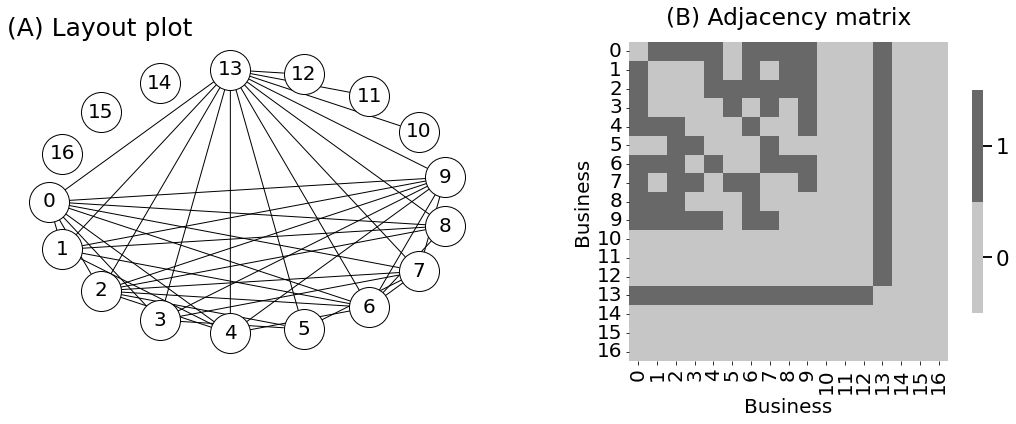
\includegraphics[width=\linewidth]{representations/ch4/Images/businessex.png}
    \caption[Business network example]{An example of a business network, where nodes are businesses and edges are whether the pairs of businesses have a business relationship.}
    \label{fig:ch4:businessex}
\end{figure}

\subsection{Node pruning}

Node pruning is a regularization technique in which you remove nodes for one reason or another. Typically, you will remove nodes due to some property about their degrees, or other properties (such as their \emph{connectedness} with other nodes that you care about). These strategies are covered loosely in the book \cite{Barabsi2013Mar}, and can be found in more computation-heavy network papers. Let's take a look at some of the strategies.

\subsubsection{Degree trimming removes nodes with unfavorable degrees}

In your business network, there are several nodes which tend to impart ``strange'' properties on downstream machine learning tasks. Some of these nodes, which include nodes with disproportionately high or low values, tend to yield numerical instability when you apply machine learning algorithms to them. By ``numerical instability'', what we mean is that the the (few) connections that nodes with low degrees have are going to have a disproportionately large impact on the machine learning task we perform. For this reason, it may be advantageous to remove nodes whose degrees are much different from the other nodes in the network. 

One special case of degree trimming is called removing \emph{isolates}. An \textit{isolated node} is a node which has a degree of $0$, meaning that it is not connected to any other nodes in the network. See if you can spot the isolates in Figure \ref{fig:ch4:businessex}.

Another special case of degree trimming is called the removal of \emph{pendants}. A \textit{pendant node} is a node which has a degree of $1$, meaning that it is only connected to one other node in the network. Try and see if you can spot the pendants in \ref{fig:ch4:businessex}.

You can remove isolates or pendants pretty simply. You simply need to compute the degree of each node in the network, and then retain the nodes with a degree \emph{above} your chosen threshold. To remove isolates, you would pick this threshold to be $0$ (retain nodes with non-zero degree), and to remove both pendants and isolates, you would pick this threshold to be $1$ (retain nodes with a degree exceeding $1$). You can do this like follows:
\begin{lstlisting}[style=python]
def compute_degrees(A):
    # compute the degrees of the network A
    # since A is undirected, you can just sum
    # along an axis.
    return A.sum(axis=1)

def prune_low_degree(A, return_inds=True, threshold=1):
    # remove nodes which have a degree under a given
    # threshold. For a simple network, threshold=0 removes isolates,
    # and threshold=1 removes pendants
    degrees = compute_degrees(A)
    non_prunes = degrees > threshold
    robj = A[np.where(non_prunes)[0],:][:,np.where(non_prunes)[0]]
    if return_inds:
        robj = (robj, np.where(non_prunes)[0])
    return robj

A_bus_lowpruned, nonpruned_nodes = prune_low_degree(A_bus)
\end{lstlisting}

Next, we'll plot the network as a layout plot. Remember how we told you in Section \ref{sec:ch4:prop-net:subnetwork} that if you just ``threw away'' nodes ignorant of which ones you threw away that you would run into trouble? Here's a good example of that. If you had just pruned the low degree nodes, you would have no idea which nodes were originally plotted \emph{where} in the initial layout plot that you looked at. Fortunately, since we included this information, we can recover the spatial position of each node pretty easily, and replot the network with the nodes that were not pruned in the same place that they were before:

\begin{lstlisting}[style=python]
node_names_lowpruned = [node_names[i] for i in nonpruned_nodes]
node_pos_lowpruned = {i : node_pos[j] for i, j in enumerate(nonpruned_nodes)}

G_bus_lowpruned = nx.from_numpy_matrix(A_bus_lowpruned)

nx.draw(G_bus_lowpruned, pos=node_pos_lowpruned)
\end{lstlisting}

The resulting layout plot is shown in Figure \ref{fig:ch4:nodeprune}(A).

\begin{figure}[h]
    \centering
    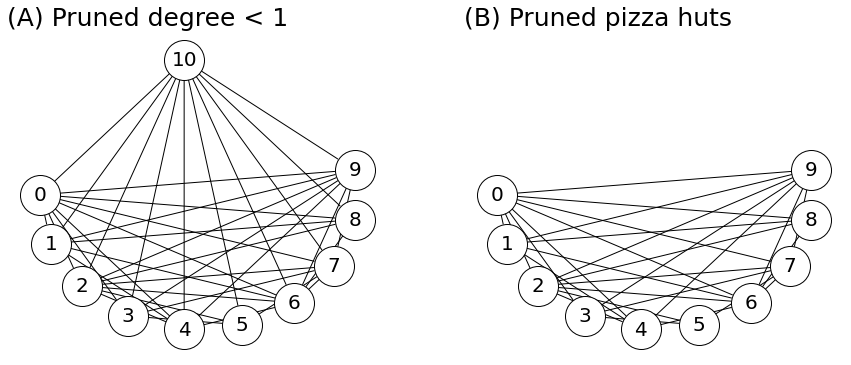
\includegraphics[width=\linewidth]{representations/ch4/Images/nodeprune.png}
    \caption[Pruning high and low degree nodes]{\textbf{(A)} The business network after pruning nodes with a degree less-than or equal to $1$, which consists of isolates and pendants. \textbf{(B)} The business network after pruning isolates and pendants followed by pizza-hut nodes.}
    \label{fig:ch4:nodeprune}
\end{figure}

A useful way to determine whether you have isolates or pendants is to look at the \emph{degree distribution histogram} of the network. The degree distribution histogram just shows a y axis of counts for a given range of possible x values. When the values you want a histogram for can only take a limited number of possible values, you might be able to get away with just looking at each possible value as its own x-axis point. Sometimes, when the values can take a large number of possible values, this might not be possible. You might have to \emph{bin} similar values together to make the plot appreciable. The degree distribution, before and after removing pendants/isolates, looks like this:

\begin{lstlisting}[style=python]
degrees_before = compute_degrees(A_bus)
degrees_after = compute_degrees(A_bus_lowpruned)
\end{lstlisting}

and can be plotted like this:

\begin{lstlisting}[style=python]
from seaborn import histplot
fig, axs = plt.subplots(1,2, figsize=(15, 4))

ax = histplot(degrees_before, ax=axs[0], binwidth=1, binrange=(0, 14))
ax.set_xlabel("Node degree");
ax.set_ylabel("Number of Nodes");
ax.set_title("Business Network, before pruning");
ax = histplot(degrees_after, ax=axs[1], binwidth=1, binrange=(0, 14))
ax.set_xlabel("Node degree");
ax.set_title("Business Network, after pruning")
\end{lstlisting}

\paragraph{Removing pizza hut nodes}

On the other end of the spectrum, it is often useful to remove nodes which don't really tell us anything about the network at all because they are just connected to \emph{everything}. We call these nodes \emph{pizza hut} nodes, because let's face it, pizza hut can be delivered pretty much anywhere! After pruning, we actually \emph{created} a pizza hut node, which you can see from low-degree pruned network in Figure \ref{fig:ch4:nodeprune}(A). 

We can prune these nodes just as easily as before. This time, note that our pruning threshold is simply set as the maximum possible node degree. Further, note that since we pruned the pizza-hut node from the low-pruned network, we need to recover which nodes from the original network were retained. This should further emphasize to you the importance of keeping track of your indices whenever you remove nodes from your network, as you can imagine that if you do a lot of node prunings, this can get confusing rapidly:

\begin{lstlisting}[style=python]
def prune_high_degree(A, return_inds=True, threshold=0):
    # remove nodes which have a degree over a given
    # threshold. For a simple network, threshold=A.shape[0] - 1
    # removes any pizza hut node
    degrees = compute_degrees(A)
    non_prunes = degrees < threshold
    robj = A[np.where(non_prunes)[0],:][:,np.where(non_prunes)[0]]
    if return_inds:
        robj = (robj, np.where(non_prunes)[0])
    return robj

# pruning nodes 
A_bus_pruned, highpruned_nodes = prune_high_degree(A_bus_lowpruned, threshold=A_bus_lowpruned.shape[0] - 1)

# get the nodes that aren't pruned by low pruning nor pizza hut node pruning
node_names_pruned = [node_names_lowpruned[i] for i in highpruned_nodes]
node_pos_pruned = {i : node_pos_lowpruned[j] for i, j in enumerate(highpruned_nodes)}

G_bus_retained = nx.from_numpy_matrix(A_bus_pruned)
nx.draw(G_bus_retained, pos=node_pos_pruned)
\end{lstlisting}
The result of both low-degree pruning (for isolates and pendants) and high-degree pruning (for pizza hut nodes) is shown in Figure \ref{fig:ch4:nodeprune}(B). 

Again, you might want to visualize the degree distribution plot to decide whether you want to prune nodes with high degrees.

\subsubsection{The Largest Connected Component is the largest subnetwork of connected nodes}

Two sections ago in Section \ref{sec:ch4:prop-net:lcc}, you learned about computing the largest connected component. This is a node pruning technique, because it "throws out" all of the nodes other than the ones which are in the largest connected component. We would encourage you to go back through this example now if you have time, so that you will better associate it as a regularization technique in your brain.


\subsection{Regularizing the edges of unweighted networks}

\subsubsection{Symmetrizing the adjacency matrix gives us undirectedness}
\label{sec:ch4:regularization:symmetrize}
If you wanted to learn from the friendship network about whether two people shared similar hobbies/activities, a reasonable first place to start might be to \emph{symmetrize} the friendship adjacency matrix. The activity/hobby network is \emph{undirected}, which means that if a student $i$ is friends on facebook with student $j$, then student $j$ is also friends with student $i$. On the other hand, as you learned above, the friendship network was directed. Since your question of interest is about an undirected network but the network you have is directed, it might be useful if you could take the directed friendship network and learn an undirected network from it. This relates directly to the concept of \emph{interpretability}, in that you need to represent your friendship network in a form that will produce an answer for us about your facebook network which you can understand.

Another reason you might seek to symmetrize the friendship adjaceny matrix is that you might think that asymmetries that exist in the adjacency matrix are just \emph{noise}. You might assume that the adjacency entries $a_{ij}$ and $a_{ji}$ relate to one another, so together they might be able to produce a single summary number that better summarizes their relationship all together. 

As a final reason, you might think that the asymmetries are meaningful, but that they \emph{are not feasible to consider}. Many statistical models for networks, and many techniques developed to analyze networks, might only have interpretations for undirected networks. This means that if you want to use these techniques, you might have to settle for making your network undirected first. 

There are many other reasons you might want undirected networks, these are just a small subset of the reasons.

Jargon wise, remember that in a symmetric matrix (for an undirected network), $a_{ij} = a_{ji}$, so in an \emph{asymmetric} matrix (for a directed network), $a_{ij} \neq a_{ji}$. To symmetrize the friendship network, what you want is a \emph{new} adjacency value, which we will call $w_{ij}$, which will be a function of $a_{ij}$ and $a_{ji}$. Then, you will construct a new adjacency matrix $A'$, where each entry $a_{ij}'$ \emph{and} $a_{ji}'$ are set equal to $w_{ij}$.  The little apostrophe just signifies that this is a potentially different value than either $a_{ij}$ or $a_{ji}$. Note that by construction, $A'$ is in fact symmetric, because $a_{ij}' = a_{ji}'$ due to how you built $A'$. For this matrix, we'll look at a generic adjacency matrix that looks like this:

\begin{align*}
    A &= \begin{bmatrix}
        a_{11} & {a_{12}} & {...} & {a_{1n}} \\
        {a_{21}} & \ddots & {\ddots} & {\vdots} \\
        {\vdots} &{\ddots} &\ddots & {a_{n-1, n}}\\
        {a_{n1}} & {...} & {a_{n,n-1}} & a_{nn}
    \end{bmatrix},
\end{align*}

\paragraph{Ignoring a ``triangle'' of the adjacency matrix}

The easiest way to symmetrize a network $A$ is to just ignore part of it entirely. In the adjacency matrix $A$, you will remember that you have an upper and a lower triangular part of the matrix. For instance, the upper triangle looks like this:

\begin{align*}
    \Delta &= \begin{bmatrix}
        0 & {a_{12}} & {...} & {a_{1n}} \\
        {0} & \ddots & {\ddots} & {\vdots} \\
        {\vdots} &{\ddots} &\ddots & {a_{n-1, n}}\\
        {0} & {...} & {0} & 0
    \end{bmatrix}.
\end{align*}
This is called the \emph{upper triangle} because if you look at the non-zero entries, they form a triangular shape in the matrix when the matrix is in its row/column orientation like this. Note this matrix is identical to $A$ for any row $i$ and column $j$ where $j > i$, but is equal to $0$ for any entries where $j \leq i$. The transpose of this matrix is:
\begin{align*}
    \Delta^\top &= \begin{bmatrix}
        0 & {0} & {...} &{0}\\
        {a_{12}}& \ddots & {\ddots} & {\vdots} \\
        {\vdots}&{\ddots} & \ddots & {0} \\
        {a_{1n}}&{...} &{a_{n-1,n}} & 0
    \end{bmatrix}.
\end{align*}
So when we add the two together, we get this:
\begin{align*}
    \Delta + \Delta^\top &= \begin{bmatrix}
        0 & {a_{12}} & {...} & {a_{1n}} \\
        {a_{12}} & \ddots & {\ddots} & {\vdots} \\
        {\vdots}&{\ddots} &\ddots & {a_{n-1, n}}\\
        {a_{1n}}&{...} &{a_{n-1,n}} & 0
    \end{bmatrix}.
\end{align*}
You're almost there! You just need to add back the diagonal of $A$, which you will do using the matrix $diag(A)$ which has values $diag(A)_{ii} = a_{ii}$, and $diag(A)_{ij} = 0$ for any $i \neq j$:
\begin{align*}
    A' &= \Delta + \Delta^\top + diag(A) = \begin{bmatrix}
        a_{11} & {a_{12}} & {...} & {a_{1n}} \\
        {a_{12}} & \ddots & {\ddots} & {\vdots} \\
        {\vdots}&{\ddots} &\ddots & {a_{n-1, n}}\\
        {a_{1n}}&{...} &{a_{n-1,n}} & a_{nn}
    \end{bmatrix},
\end{align*}
which leaves $A'$ to be a matrix consisting \emph{only} of entries which were in the upper right triangle of $A$. $A'$ is obviously symmetric, because $a_{ij}' = a_{ji}'$ for all $i$ and $j$. Since the adjacency matrix is symmetric, the network $A'$ represents is undirected.

\begin{floatingbox}[h]
\caption{When is ``ignoring'' a triangle appropriate?}

When you have an undirected network, it is often the case that the network will be stored only as a single ``triangle'' with the diagonal, since half of the matrix is redundant. Therefore, you can save potentially a lot of space by only storing a little over half of it (a little over because, you need to retain the one triangle + the diagonal, and not just a triangle). So if you want the actual adjacency matrix, you need to ``ignore'' the uninformative triangle, and ``retain'' the informative one, like the procedure above.
\end{floatingbox}


So what does this mean in terms of the network itself? This means that the network originally had edge weights $a_{ij}$, where $a_{ij}$ might not be equal to $a_{ji}$. Let's consider this in terms of the activity/hobby network. The activity/hobby network, which is undirected, perhaps has been stored in a representation where the entire lower-left triangle is just zeros, for space purposes. When you then upper-right symmetrize it, the network looks like this, using the \texttt{graspologic} function \texttt{symmetrize} with \texttt{method="triu"} (upper triangular symmetrization):


\begin{lstlisting}[style=python]
from graspologic.utils import symmetrize

# upper-triangle symmetrize the upper triangle
A_activity = symmetrize(A_activity_uppertri, method="triu")
\end{lstlisting}
We plot the two heatmaps in Figure \ref{fig:ch4:triusym}.

\begin{figure}[h]
    \centering
    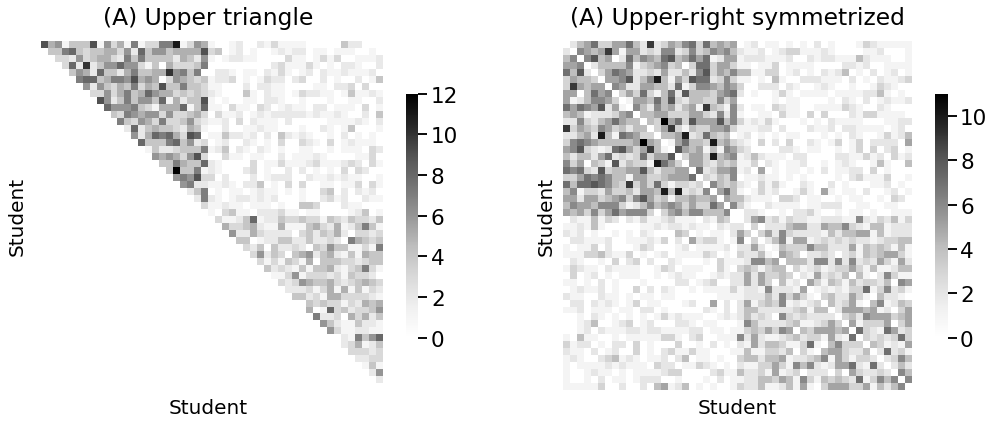
\includegraphics[width=\linewidth]{representations/ch4/Images/triusym.png}
    \caption[Symmetrization through discarding a triangle]{The matrices \texttt{A\_activity\_uppertri} and \texttt{A\_activity\_triu\_symmetrized} showing the \textbf{(A)} upper triangle, \textbf{(B)} and upper-right symmetrized adjacency matrices.}
    \label{fig:ch4:triusym}
\end{figure}
Likewise, if the network only had the lower triangle stored, you could do the same thing but with\texttt{method="tril"} to retain the lower triangle of the matrix.

\paragraph{Taking a function of the two values}

There are many other ways you use a function of $a_{ij}$ and $a_{ji}$ to get a symmetric matrix (and an undirected network). One is to just average. That is, you can let the matrix $A'$ be the matrix with entries $a'_{ij} = \frac{a_{ij} + a_{ji}}{2}$ for all $i$ and $j$. In matrix form, this operation looks like this:

\begin{align*}
    A' &= \frac{1}{2} (A + A^\top) \\
    &= \frac{1}{2}\left(\begin{bmatrix}
        a_{11} & ... & a_{1n} \\
        \vdots & \ddots & \vdots \\
        a_{n1} & ... & a_{nn}
    \end{bmatrix} + \begin{bmatrix}
        a_{11} & ... & a_{n1} \\
        \vdots & \ddots & \vdots \\
        a_{1n} & ... & a_{nn}
    \end{bmatrix}\right)\\
    &= \begin{bmatrix}
        \frac{1}{2}(a_{11} + a_{11}) & ... & \frac{1}{2}(a_{1n} + a_{n1}) \\
        \vdots & \ddots & \vdots \\
        \frac{1}{2} (a_{n1} + a_{1n}) & ... & \frac{1}{2}(a_{nn} + a_{nn})
    \end{bmatrix} \\
    &= \begin{bmatrix}
        a_{11} & ... & \frac{1}{2}(a_{1n} + a_{n1}) \\
        \vdots & \ddots & \vdots \\
        \frac{1}{2} (a_{n1} + a_{1n}) & ... & a_{nn}
    \end{bmatrix}
\end{align*}
As you can see, for all of the entries, $a'_{ij} = \frac{1}{2} (a_{ij} + a_{ji})$, and also $a_{ji}' = \frac{1}{2}(a_{ji} + a_{ij})$. These quantities are the same, so $a_{ij}' = a_{ji}'$, and $A'$ is symmetric. As the adjacency matrix is symmetric, the network that $A'$ represents is undirected.

Remember that the asymmetry in the friendship network means student $i$ might perceive their friendship with student $j$ as being stronger or weaker than student $j$ perceived about student $i$. What you did here was instead of just arbitrarily throwing one of those values away, you said that their friendship might be better indicated by averaging the two values. This produced for us a single friendship strength $a_{ij}'$ where $a_{ij}' = a_{ji}'$.

You can implement this in graspologic as follows:
\begin{lstlisting}[style=python]
# symmetrize with averaging
A_friend_avg_sym = symmetrize(A_friend, method="avg")
\end{lstlisting}
We'd encourage you to plot the outcome and convince yourself that it is, in fact, symmetric using the \texttt{is\_symmetric()} function you learned about in the last section.

We'll will use the friendship network symmetrized by averaging (\texttt{A\_friend\_avg\_sym}) in several of the below examples, which we will call the ``undirected friendship network''.

\subsubsection{Diagonal augmentation}
\label{sec:ch4:regularization:diag_aug}

In your future works with network machine learning, you will come across numerous techniques which operate on adjacency matrices which are \emph{positive semi-definite}. This word doesn't need to mean a whole lot to you conceptually, but it has a big implication when you try to use algorithms on many of your networks. Remember that when you have a loopless network, a common practice in network science is to set the diagonal to zero. What this does is it leads to your adjacency matrices being \emph{indefinite} (which means, \emph{not} positive semi-definite). For our purposes, this means that many network machine learning techniques simply cannot operate on these adjacency matrices. However, as we mentioned before, these entries are not actually zero, but simply \emph{do not exist} and you just didn't have a better way to represent them. Or do you?

\emph{Diagonal augmentation} is a procedure for imputing the diagonals of adjacency matrices for loopless networks. This gives us "placeholder" values that do not cause this issue of indefiniteness, and allow your network machine learning techniques to still work. Remember that for a simple network, the adjacency matrix will look like this:
\begin{align*}
    A &= \begin{bmatrix}
        0 & a_{12} & ... & a_{1n} \\
        a_{21}& \ddots & & \vdots \\
        \vdots & & \ddots & a_{n-1, n} \\
        a_{n1} &...& a_{n, n-1} & 0
    \end{bmatrix}
\end{align*}

What you do is impute the diagonal entries using the \emph{fraction of possible edges which exist} for each node. This quantity is simply the node degree $d_i$ (the number of edges which exist for node $i$) divided by the number of possible edges node $i$ could have (which would be node $i$ connected to each of the other $n-1$ nodes). Remembering that the degree matrix $D$ is the matrix whose diagonal entries are the degrees of each node, the diagonal-augmented adjacency matrix is given by:
\begin{align*}
    A' &= A + \frac{1}{n-1}D = \begin{bmatrix}
        \frac{d_1}{n-1} & a_{12} & ... & a_{1n} \\
        a_{21}& \ddots & & \vdots \\
        \vdots & & \ddots & a_{n-1, n} \\
        a_{n1} &...& a_{n, n-1} & \frac{d_n}{n-1}
    \end{bmatrix}
\end{align*}
When the matrices are directed or weighted, the computation is a little different, but fortunately \texttt{graspologic} will handle this for us. Let's see how you would apply this to the directed friendship network:
\begin{lstlisting}[style=python]
from graspologic.utils import augment_diagonal

A_friend_aug = augment_diagonal(A_friend)
\end{lstlisting}
We will rotate back to the problem of positive semi-definiteness in Section \ref{sec:ch5:psd_block} as it relates to statistical models for networks, and will pivot back again in Section \ref{sec:ch6:spectral} for what it means with regard to adjacency matrices.

\subsection{Regularizing the edges of weighted networks}

As you are probably aware, in all of machine learning, you are always concerned with the \emph{bias/variance tradeoff}. The \textit{bias/variance tradeoff} is an unfortunate side-effect that concerns how well a learning technique will generalize to new datasets \cite{Hastie2009}.
\begin{enumerate}
    \item \textit{Bias} is an error from erroneous assumptions you make about the system that you are learning about. For instance, if you have a friendship network, you might make simplifying assumptions, such as an assumption that two athletes frorm different sports have an equally likely chance of being friends with a member of the band. This might be flat out false, as band members might be selectively better friends with athletes depending on which sports they play.
    \item On the other hand, the \textit{variance} is the degree to which the an estimate of a task will change when given new data. An assumption that if a player is a football player he has a higher chance of being friends with a band member might make sense given that the band performs at football games. 
\end{enumerate}

The "trade-off" is that these two factors tend to be somewhat at odds, in that raising the bias tends to lower the variance, and vice-versa:
\begin{enumerate}
    \item \textit{High bias, but low variance}: Whereas a lower variance model might be better suited to the situation where the data you expect to see is noisy, it might not as faithfully represent the underlying dynamics you think the network possesses. A low variance model might ignore that athletes might have a different chance of being friends with a band member based on their sport all together. This means that while you won't get the student relationships \emph{correct}, you might still be able to get a reasonable estimate that you think is not due to overfitting. In this case, you've smoothed away \emph{signal} from the data at the expense of avoiding \emph{noise}.
    \item \textit{Low bias, but high variance}: Whereas a low bias model might more faithfully model true relationships in your training data, it might fit your training data a little \emph{too} well. Fitting the training data too well is a problem known as \textit{overfitting}. If you only had three football team members and tried to assume that football players were better friends with band members, you might not be able to well approximate this relationship because of how few individuals you have who reflect this situation. 
\end{enumerate}

Here, we show several strategies to reduce the variance (but, add bias) due to edge weight noise in network machine learning.

\subsubsection{Sparsification of the network}

The procedure of \textit{sparsification} is one in which we take a network, and we remove edges from it, which is described by \cite{Spielman2008Aug} and \cite{Batson2013Aug}. Remember that removing edges, in terms of the adjacency matrix, is analogous to setting the corresponding adjacencies to zero. A matrix with many entries of zero is called a \emph{sparse} matrix. So, the reason we call the removal of the edges from a network \emph{sparsification} is that we are producing a network with a \emph{sparse} adjacency matrix.

\emph{Sparsification} is a general class of edge regularization techniques, and includes many flavors. Here, we discuss a few of them. In network sparsification, we will often pick some property of the network (such as, a particular edge weight) and remove edges in an attempt to preserve something about this particular property.

A useful tool to study for how, exactly, you might want to go about sparsifying the network is called the \emph{edge-weight distribution} of your network sample. The edge-weight distribution of the network sample are the particular values that the edge weights of the network take. The most common way to visualize the edge-weight distribution is an edge-weight histogram. This is very similar to the node-degree histogram you worked with above, but instead of node degrees, you look at the edge-weights. Let's take a look at the friendship network, and then take a look at its edge-weight distribution. Remember that the friendship network is \emph{undirected}, so we need to remove its diagonal elements \emph{before} we visualize the edge-weight distribution. We'll also remove edges with zero-weights for visualization purposes:

\begin{lstlisting}[style=python]
def discard_diagonal(A):
    """
    A function that discards the diagonal of a matrix,
    and returns its non-diagonal edge-weights.
    """
    # create a mask that is True for the non-diagonal edges
    non_diag_idx = np.where(~np.eye(A.shape[0], dtype=bool))
    return A[non_diag_idx].flatten()

friend_nondiag_ew = discard_diagonal(A_friend)
# get the non-zero, non-diagonal edge weights
friend_nondiag_nz_ew = friend_nondiag_ew[friend_nondiag_ew > 0]

# plot the histogram, as above
histplot(friend_nondiag_nz_ew, bins=20, binrange=(0, 1))
\end{lstlisting}
We show this plot in Figure \ref{fig:ch4:truncate}(C).

\begin{figure}[h]
    \centering
    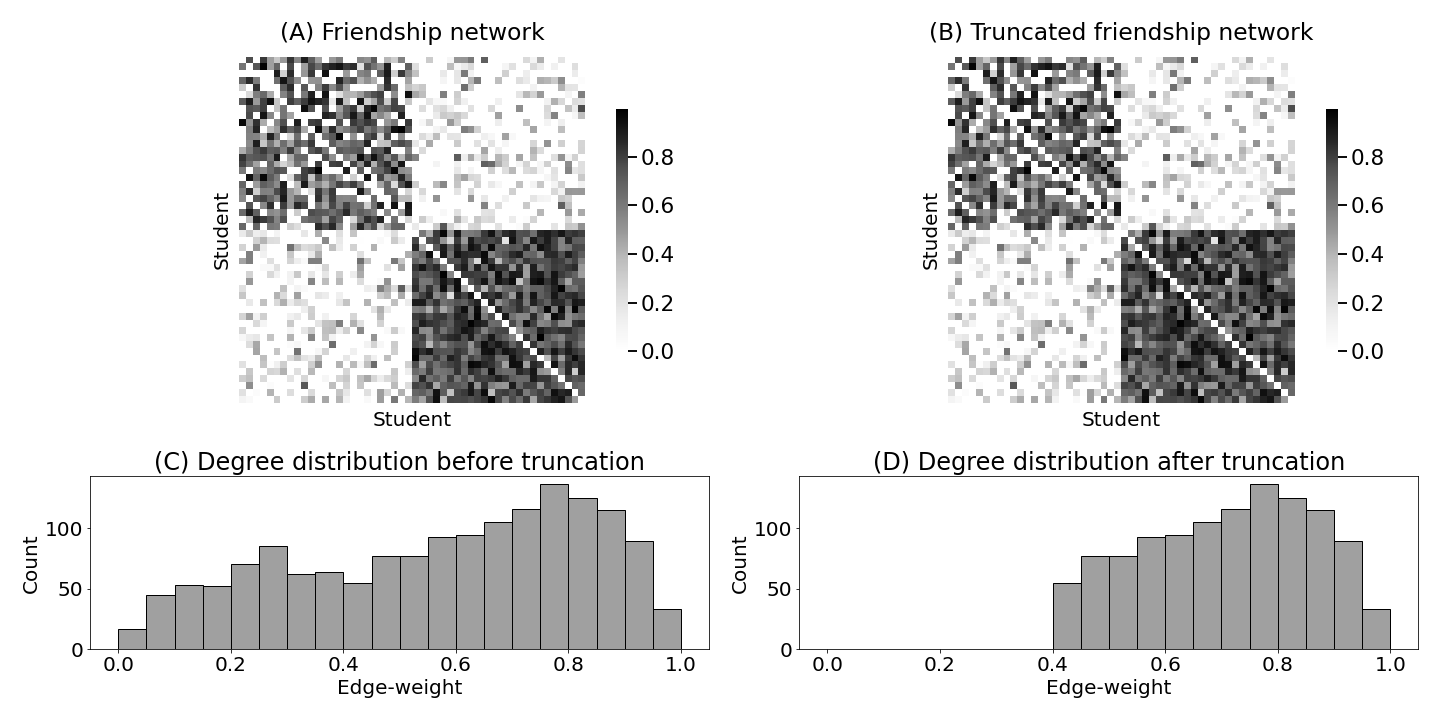
\includegraphics[width=\linewidth]{representations/ch4/Images/truncate.png}
    \caption[Truncation]{\textbf{(A)} The adjacency matrix before truncation. \textbf{(B)} The adjacency matrix after truncation. \textbf{(C)} The non-zero, non-diagonal edge weights before truncation. \textbf{(D)} The non-zero, non-diagonal edge weights after truncation.}
    \label{fig:ch4:truncate}
\end{figure}

\paragraph{Truncation removes the smallest edges}

The simplest way to reduce the variance due to edge weight noise is called \emph{edge truncation}. \textit{Edge truncation} is a process by which you choose some threshold value $\tau$, and remove all of the weights which are smaller than $\tau$ but retain the weights that are bigger than $\tau$. For edges that are equal to $\tau$, what you'll want to do depends on the strategy you are employing. We'll arbitrarily set nodes $\leq \tau$ to zero in our case, but you might use $\geq \tau$ in your uses.

So, how is $\tau$ typically chosen? There are a few ways, but it's usually one of the below two:
\begin{enumerate}
    \item Choose $\tau$ arbitrarily: after looking at your network and doing some preliminary visualizations, you might determine that your edge weights tend to be ``multi-modal''. This means that when you look at the edge-weight distribution, you see multiple "clusters" of edge weight bins which are larger, or smaller. For a lot of networks, these small edges might be very noise induced; that is, the small edges might just spuriously be close to, but {not quite}, zero, due to errors in your measuring process. When the edge weights are really tiny, you might think that these noisy edges are better off just not existing.
    \item Choose $\tau$ based on a particular quantile: A \textit{quantile} is a percentile divided by $100$. In this strategy, you identify a target quantile of the edge-weight distribution. What this means is that you are selecting the lowest {fraction} of the edge-weights (where that fraction is the quantile that you choose) and setting these edges to $0$, and selecting the remaining edges are left unchanged. If you select a quantile of $0.5$, this means that you take the smallest $50\%$ of edges and set them to zero, and the largest $50\%$ of edges and retain their initial value. There are three potential pitfalls to quantiling, which we elaborate on below.
\end{enumerate}
This is called \emph{truncation} because you are taking the edge-weight distribution, and \emph{truncating} (cutting it off) below the value $\tau$.

With respect to what to do with edges that are equal to $\tau$, when you choose a threshold arbitrarily, you can do whatever you want with them, as long as you are consistent if you have multiple networks you are truncating. What we mean by this is that you can select to remove edges less than or equal to this threshold, or retain edge weights greater than or equal to the threshold. When you truncate on the basis of a quantile, however, this is not quite the case. You will want to remove all the edges below $\tau$, and truncate away the remaining edges equal to $\tau$ at random until you have truncated the desired fraction of edges in total.

Let's see how this works in practice. In the edge-weight histogram, in Figure \ref{fig:ch4:truncate} you can notice two "peaks" to the non-zero edge-weights.

If you think that the smaller peak edge-weights are spurious/noise, you might want to threshold somewhere in between the smaller and the larger peaks, like near $0.4$, which is highlighted in \ref{fig:ch4:truncate}(C). 

\begin{lstlisting}[style=python]
def truncate_network(A, threshold):
    A_cp = np.copy(A)
    A_cp[A_cp <= threshold] = 0
    return A_cp

tau = 0.4
A_friend_trunc = truncate_network(A_friend, threshold=tau)
\end{lstlisting}
The next thing to look at is the adjacency matrix, before and after truncation. We show these plots in Figure \ref{fig:ch4:truncate}(A) and \ref{fig:ch4:truncate}(B). Notice that the smallest weight edges in the network (in this case, the ones with edge weights $\leq 0.4$) have been replaced with zeros. As you can see, a lot of the edges in the upper right and upper left, which were previously small, are now \emph{zero}. This is reflected in the edge-weight distribution:

\begin{lstlisting}[style=python]
friend_trunc_nondiag_ew = discard_diagonal(A_friend_trunc)
# get the non-zero, non-diagonal edge weights
friend_trunc_nondiag_nz_ew = friend_trunc_nondiag_ew[friend_trunc_nondiag_ew > 0]
histplot(friend_trunc_nondiag_nz_ew, bins=20, binrange=(0, 1))
\end{lstlisting}
which is shown in Figure \ref{fig:ch4:truncate}(D). As you can see, all of the edges with weights less than $\tau = 0.4$ have been truncated away.

A slight caveat to this procedure we learned about above for truncation is that, if you use the quantile approach and the network is undirected, you need to exclude one triangle of the network to obtain the appropriate quantile. This is because when $a_{ij} = a_{ji}$, you would otherwise count an edge twice if you just used the adjacency matrix to obtain quantiles. We'll see this more in the example on thresholding below.


\paragraph{Thresholding converts weighted networks to unweighted networks}
\label{sec:ch4:regularization:thresholding}

Closely related to truncation is the process of \emph{thresholding}. Like truncation, you begin with a threshold $\tau$, which is usually chosen arbitrarily or based on a quantile, like for truncation. However, there is one key difference: when you threshold a network, you set the edges below $\tau$ to zero, and the edges greater than $\tau$ to \emph{one}. This has the effect of taking a weighted network, and effectively transforming it into an undirected network. 

We will show how to use the quantile approach to thresholding, with the activity/hobby network. You will threshold by choosing $\tau$ such that $\tau$ is the value which is the $0.3$ quantile, or the $30$ percentile, of the edge-weight distribution. Remember as you learned in the preceding section, that if the network itself is loopless, the diagonal entries simply \emph{do not exist}; $0$ is simply a commonly used placeholder. For this reason, when you compute quantiles of edge-weights, you need to \emph{exclude the diagonal} if the network is loopless. 

\begin{floatingbox}[h]\caption{Why is thresholding with a quantile desirable?}\label{box:ch4:desirable}
Remember that in Section \ref{sec:ch4:prop-net:density}, we defined the network density for a simple network as:

\begin{align*}
    density(A) &= \frac{\sum_{j > i}a_{ij}}{\binom{n}{2}}.
\end{align*}

If you threshold this network at a quantile of $q$, this means you will, ideally, set $1 - q$ fraction of the edges to $1$, and a $q$ fraction of the edges to zero.

If we are able to do this perfectly, then $\sum_{j > i}a_{ij} = (1 - q)\binom n 2$.

Therefore:
\begin{align*}
    density(A) &= \frac{(1 - q)\binom n 2}{\binom n 2} = 1 - q
\end{align*}

So when you threshold the network at a quantile $q$, and you are {actually} able to set a $q$ fraction of the edges to zero and a $1 - q$ fraction of the edges to one, you end with a network of density equal to $1 - q$. We will see a for conditions as to when this will, and will not, occur later.
\end{floatingbox}

Further, since this network is undirected, you also need to restrict your attention to one triangle of the corresponding adjacency matrix. We choose the upper-right triangle arbitrarily, as the adjacency matrix's symmetry means the upper-right triangle and lower-right triangle have identical edge-weight distributions. We can do this using \texttt{numpy}. This network is loopless and undirected, so we will want to exclude both the diagonal {and} only perform our analysis on a single triangle of the matrix:
\begin{lstlisting}[style=python]
# find the indices which are in the upper triangle and not in the diagonal
upper_tri_non_diag_idx = np.where(np.triu(np.ones(A_activity.shape), k=1).astype(bool))
q = 0.3  # desired quantile is 0.5, or 50 percentile
histplot(A_activity[upper_tri_non_diag_idx].flatten())
tau = np.quantile(A_activity[upper_tri_non_diag_idx], q=q)
\end{lstlisting}

So, let's see what happens when we just compute $\tau$ using the $q$ quantile of the non-diagonal, upper triangular entries of $A$, and then threshold $A$ using $\tau$. To do this, we'll just check the number of edges greater than $\tau$, and the number less than or equal to $\tau$. Since we used $q = 0.5$ as our desired quantile, we should anticipate that these numbers should be very close to equal:

\begin{lstlisting}[style=python]
n_lteq_tau = np.sum(A_activity[upper_tri_non_diag_idx] <= tau)
n_gt_tau = np.sum(A_activity[upper_tri_non_diag_idx] > tau)
print("Number of edges less than or equal to tau: {}".format(n_lteq_tau))
print("Number of edges greater than to tau: {}".format(n_gt_tau))
\end{lstlisting}
While the specific results you obtain will depend on your specific computer since we used random simulation data here, you're going to get numbers that are not even close to equal (the number of edges $\leq \tau$ should be about 50\% larger than the number of edges $> \tau$). So what happened?

\paragraph{The duplicate value pitfall}

Let's imagine an array that was \texttt{[1,2,3,4]} and \texttt{[1,2,2,4]}, and we chose the $0.5$ quantile, the first array would give a $0.5$ quantile of \texttt{2.5}. If we thresholded with this value, we would get \texttt{[0,0,1,1]}, and the number of elements retained after thresholding would be $50\%$ ones and $50\%$ zeros, like we expected. On the other hand, the $0.5$ quantile of the second array is \texttt{2}, and if we used the thresholding approach above we would get \texttt{[0,0,0,1]}, which has $75\%$ of the values taking $0$ and $25\%$ of the values taking one. 

This means that if you pass in a quantile $q$ and you expect that $q$ fraction of the points will have a value of $0$ after truncation/thresholding, you are going to need to be very careful with your data to handle points that are \emph{equal} to your quantile. To do this, one way is to assign edges less than $\tau$ to zero, and the edges greater than $\tau$ to one. Then, for edges equal to $\tau$, you can to randomly assign them to a zero or one, until you obtain the desired quantiling threshold. This can be done with the pseudocode in Algorithm \ref{alg:ch4:thresholding}. You could write a similar utility for truncating at a quantile.

\begin{algorithm}[h]
    \SetAlgoLined
    \caption{Thresholding an adjcency matrix with random tiebreaking.}
    \label{alg:ch4:thresholding}
    \KwData{$A$: an adjacency matrix \newline $q$: a quantile between $0$ and $1$}
    \KwResult{an adjacency matrix thresholded at the $q$ quantile.}
    Let $d$ be the minimum non-zero difference between any two elements of $A$.
    
    \For{$i$ in $1$ : $n$}{
        \For{$j$ in $1$ : $n$}{
            Let $\epsilon_{ij}$ be a random number between $0$ and $d$.
        }
    }

    \If{$A$ is symmetric}{
        $\epsilon = \frac{\epsilon + \epsilon^\top}{2}$
    }

    Compute the augmented adjacency matrix, $A' = A + \frac{\epsilon}{10}$.

    Compute the appropriate threshold $\tau$ using $A'$.

    Threshold $A'$ by setting elements where $a_{ij}' > \tau$ to one, and $a_{ij}' < \tau$ to zero.
\end{algorithm}

Basically, what this algorithm does is it adds a very small amount of noise to the matrix $A$ that you are thresholding. Note that we take care to ensure that if $A$ is symmetric and the network is undirected, that we add the \emph{same} amount of noise to both entries $a_{ij}$ and $a_{ji}$ by \emph{symmetrizing} this ``noise matrix'' $\epsilon$. This noise is small enough that it is an order of magnitude (a factor of $10$) smaller than the smallest appreciable difference in any two non-zero elements of $A$. 

After we add this matrix to $A$, there is a probability of \emph{zero} that any two elements of $A$ will have the same value. Further, since we added noise that was an order of magnitude smaller than any non-zero differences of elements of $A$, it is impossible for an item that was originally greater than a quantile to now be less than the desired quantile, and vice-versa. This strategy is called a random tiebreaking, since we broke ties that occur at exactly the $q$ quantile randomly.

This can be implemented in python as follows:

\begin{lstlisting}[style=python]
from numpy import copy

def min_difference(arr):
    b = np.diff(np.sort(arr))
    return b[b>0].min()

def quantile_threshold_network(A, directed=False, loops=False, q=0.5):
    # a function to threshold a network on the basis of the
    # quantile
    A_cp = np.copy(A)
    n = A.shape[0]
    E = np.random.uniform(low=0, high=min_difference(A)/10, size=(n, n))
    if not directed:
        # make E symmetric
        E = (E + E.transpose())/2
    mask = np.ones((n, n))
    if not loops:
        # remove diagonal from E
        E = E - np.diag(np.diag(E))
        # exclude diagonal from the mask
        mask = mask - np.diag(np.diag(mask))
    Ap = A_cp + E
    tau = np.quantile(Ap[np.where(mask)].flatten(), q=q)
    A_cp[Ap <= tau] = 0; A_cp[Ap > tau] = 1
    return A_cp

A_activity_thresholded03 = quantile_threshold_network(A_activity, q=0.3)
A_activity_thresholded07 = quantile_threshold_network(A_activity, q=0.7)
\end{lstlisting}
We visualize these two thresholded adjacency matrices along with the unweighted adjacency matrix in Figure \ref{fig:ch4:threshold_res}.

\begin{figure}[h]
    \centering
    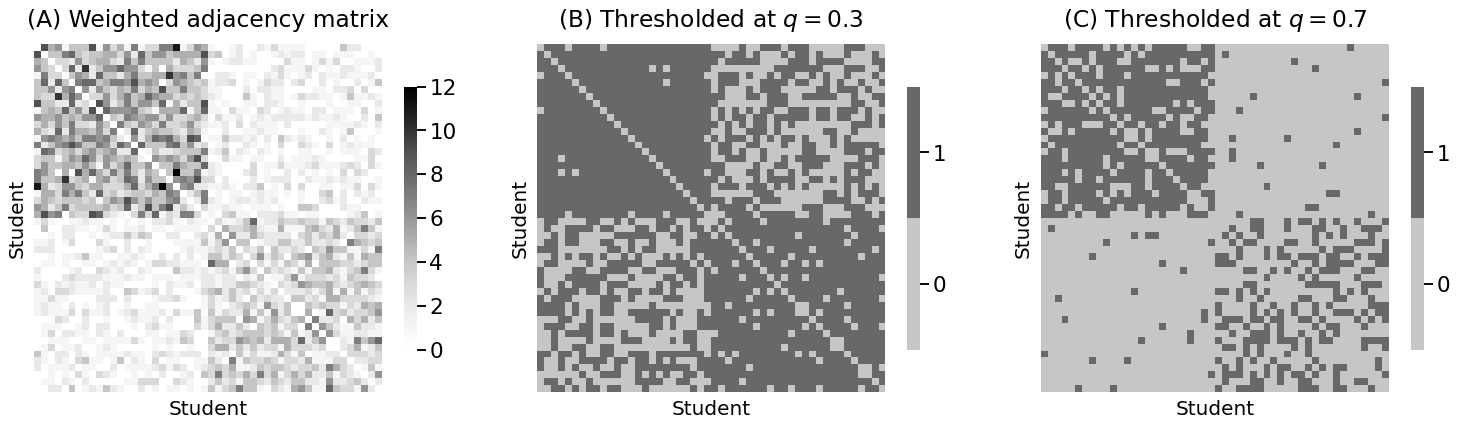
\includegraphics[width=\linewidth]{representations/ch4/Images/threshold_res.png}
    \caption[Thresholding]{\textbf{(A)} the weighted adjacency matrix of the activity/hobby network. \textbf{(B)} the weighted adjacency matrix of the activity/hobby network after thresholding at $0.3$. \textbf{(C)} the weighted adjacency matrix of the activity/hobby network after thresholding at $0.7$.}
    \label{fig:ch4:threshold_res}
\end{figure}

Great job. Now, let's just confirm that we didn't run into the duplicate value pitfall. We'll do this by writing a utility which computes the network density from an adjacency matrix for a simple network:

\begin{lstlisting}[style=python]
from graspologic.utils import is_unweighted, is_loopless, is_symmetric

def simple_network_dens(X):
    # make sure the network is simple
    if (not is_unweighted(X)) or (not is_loopless(X)) or (not is_symmetric(X)):
        raise TypeError("Network is not simple!")
    # count the non-zero entries in the upper-right triangle
    # for a simple network X
    nnz = np.triu(X, k=1).sum()
    # number of nodes
    n = X.shape[0]
    # number of possible edges is 1/2*n*(n-1)
    poss_edges = 0.5*n*(n-1)
    return nnz/poss_edges

print("Network Density: {:.3f}".format(simple_network_dens(A_activity_thresholded03)))
# Network Density: 0.700
\end{lstlisting}

So our solution achieved the desired network density.

We call this pitfall the \emph{duplicate value pitfall} because you can \emph{only} run into it if your adjacency matrix has the same value duplicated.

\paragraph{The ``underly ambitious'' pitfall}

The next pitfall of using a quantile $q$ is actually a special case of the duplicate value pitfall listed above: you might choose an underly ambitious quantile to truncate/threshold with. By underly ambitious, what we mean is that the adjacency matrix doesn't even have a $1 - q$ fraction of non-zero edges. When you threshold $A$ with a quantile of $q$, you can spot this pitfall fairly easily by simply checking the fraction of $0$-weight edges ahead of time.

For an example, let's consider a network where $50\%$ of the possible edges are zero (the network density is $0.5$, and the other $50\%$ are one. If you were to choose a quantile of $0.3$, quantiling will still only give you a network density of $0.5$, and not $0.7$ like you might have expected from Remark \ref{box:ch4:desirable}.

Unfortunately, there's no quick fix like there was for the non-continuous pitfall; if you run into the underly ambitious pitfall and tried to use the randomization procedure, the ``solution'' would end up setting edges with a value of zero in the adjacency matrix to one, which doesn't make much sense. To avoid this pitfall, you need to analyze your densities ahead of time if you want to use quantiling, and ensure that the quantile you choose is not underly ambitious. 

If you had a collection of networks that you wanted to threshold or truncate \emph{en masse} using a quantile $q$, you could do this by plotting a histogram of your network densities, and ensuring that $1 - q$ is less than all of the network densities in your collection.

\begin{floatingbox}[h]\caption{With all these pitfalls, why would we quantile?}
As we mentioned in Section \ref{sec:ch4:net-rep:featurelims}, many network summary statistics that you might be interested in could be heavily correlated with the network density. For this reason, if you want to analyze a collection of networks using summary statistics, it might make sense to analyze a collection of networks with the same network density. This is because in some sense, analyzing the networks with a similar network density will ``decouple'' this correlation with the network density, since the network density will no longer be changing across the networks.
\end{floatingbox}

\paragraph{When can we ignore these pitfalls entirely?}

As you might be able to gather from the above, if our network fulfills two properties, we are guaranteed that we won't run into the quantiling pitfalls. First, if the network is \textit{dense} (a network where all possible entries $a_{ij}$ are non-zero, with arbitrarily small or large edge-weights), we cannot possibly run into the underly ambitious pitfall, since that pitfall will only arise when there are zero-weight edges in the adjacency matrix. Second, if the adjacency matrix does not have any duplicate values, we cannot run into the duplicate value pitfall either, because we cannot have ties at the desired quantile if there are no duplicated values in the edge weights. 

As we have repeated many times in this section, when considering when a network might run into these pitfalls using the adjacency matrix, be sure to only consider appropriate entries of the adjacaency matrix. This means restricting your analysis to the upper triangle or the lower triangle if the netework is undirected, and removing the diagonal if the network is loopless. 

\subsubsection{Edge-weight global rescaling}

With weighted networks, it is often the case that you might want to reshape the distributions of edge-weights in your networks to highlight particular properties. Notice that the edge-weights for your friendship network takes values between $0$ and $1$, but your activity network takes values between $0$ and almost $15$. How can you possibly compare between these two networks where the edge-weights take such different ranges of values? You turn to standardization, which allows us to place values from different networks on the same scale. 

\paragraph{$z$-scoring standardizes edge weights using the normal distribution}

The first approach to edge-weight standardization is known commonly as $z$-scoring. Suppose that $A$ is the adjacency matrix, with entries $a_{ij}$. With a $z$-score, you will rescale the weights of the adjacency matrix, such that the new edge-weights (called $z$-scores) are approximately normally distributed. The reason this can be useful is that the normal distribution is pretty ubiquitous across many branches of science, and therefore, a $z$-score is relatively easy to communicate with other scientists. Further, many things that exist in nature can be well-approximated by a normal distribution, so it seems like a reasonable place to start to use a $z$-score for edge-weights, too! The $z$-score is defined as follows. You will construct the $z$-scored adjacency matrix $Z$, whose entries $z_{ij}$ are the corresponding $z$-scores of the adjacency matrix's entries $a_{ij}$. For a weighted, loopless network, you use an estimate of the \emph{mean}, $\hat \mu$, and the \emph{unbiased} estimate of the \emph{variance}, $\hat \sigma^2$, which can be computed as follows:
\begin{align*}
    \hat\mu &= \frac{1}{n(n-1)}\sum_{i \neq j}a_{ij},\\
    \hat\sigma^2 &= \frac{1}{n(n - 1) - 1}\sum_{i \neq j} (a_{ij} - \hat\mu)^2.
\end{align*}
The $z$-score for the $(i,j)$ entry is simply the quantity:
\begin{align*}
    z_{ij} &= \frac{a_{ij} - \hat\mu}{\hat\sigma}
\end{align*}
Since your network is loopless, notice that these sums are for all \emph{non-diagonal} entries where $i \neq j$. If the network were not loopless, you would include diagonal entries in the calculation, and instead would sum over all possible combinations of $i$ and $j$. the interpretation of the $z$-score $z_{ij}$ is the \emph{number of stadard deviations} that the entry $a_{ij}$ is from the mean, $\hat \mu$.

We will demonstrate on the directed friendship network. You can implement $z$-scoring as follows:

\begin{lstlisting}[style=python]
from scipy.stats import zscore

def z_score_loopless(X, undirected=False):
    if not is_loopless(X):
        raise TypeError("The network has loops!")
    if is_symmetric(X):
        raise TypeError("The network is undirected!")
    # the entries of the adjacency matrix that are not on the diagonal
    non_diag_idx = np.where(~np.eye(X.shape[0], dtype=bool))
    Z = np.zeros(X.shape)
    Z[non_diag_idx] = zscore(X[non_diag_idx])
    return Z

ZA_friend = z_score_loopless(A_friend)
\end{lstlisting}

The theory for when, and why, to use $z$-scoring for network machine learning tends to go something like this: many things tend to be normally distributed with the same mean and variance, so perhaps that is a reasonable expectation for your network, too. Unfortunately, we find this often to \emph{not} be the case. In fact, we often find that the specific distribution of edge weights itself often might be lamost infeasible to identify in a population of networks, and therefore \emph{almost} irrelevant all-together. To this end, we turn to instead \emph{ranking} the edges.

Note that in the above code snippet, we throw an error if the network is undirected (and the adjacency matrix is symmetric): remember that you want to be careful to restrict your analysis to the upper triangle if the network is undirected and loopless. This won't really change the estimate of the mean, but the variance will be slightly different. The sums would be over $j > i$, and the normalizing factors would be $\binom n 2$ instead of $n(n - 1)$.

\paragraph{Ranking edges preserves ordinal relationships}

The idea behind ranking is as follows. You don't really know much useful information as to how the distribution of edge weights varies between a given pair of networks. For this reason, you want to virtually eliminate the impact of that distribution \emph{almost} entirely. However, you know that if one edge-weight is larger than another edge-weight, that you do in fact trust that relationship. What this means is that you want something which preserves \emph{ordinal} relationships in your edge-weights, but ignores other properties of the edge-weights. An ordinal relationship just means that you have a natural ordering to the edge-weights. This means that you can identify a largest edge-weight, a smallest edge-weight, and every position in between. When we want to preserve ordinal relationships in your network, we do something called \emph{passing the non-zero edge-weights to ranks}. We will often use the abbreviation\texttt{ptr} to define this function because it is so useful for weighted networks. We pass non-zero edge-weights to ranks as in Algorithm \ref{alg:ch4:ptr}.

\begin{algorithm}[h]
    \SetAlgoLined
\caption{Passing an adjacency matrix to ranks}
\label{alg:ch4:ptr}
    \KwData{$A$ is an adjacency matrix.}
    \KwResult{The adjacency matrix, after passing to ranks.}
    Identify all of the non-zero entries of the adjacency matrix $A$.

    Let $n_{nz}$ be the number of non-zero entries of the adjacency matrix $A$.

    Rank all of the non-zero edges in the adjacency matrix $A$, where for a non-zero entry $a_{ij}$, $rank(a_{ij}) = 1$ if $a_{ij}$ is the smallest non-zero edge-weight, and $rank(a_{ij}) = n_{nz}$ if $a_{ij}$ is the largest edge-weight. Ties are settled by using the average rank of the tied entries.

    Report the weight of each non-zero entry $(i,j)$ as $r_{ij} = \frac{rank(a_{ij})}{n_{nz} + 1}$, and for eachh zero entry as $r_{ij} = 0$.
\end{algorithm}

Below, we pass-to-ranks the directed friendship network using\texttt{graspologic}:

\begin{lstlisting}[style=python]
from graspologic.utils import pass_to_ranks

RA_friend = pass_to_ranks(A_friend)
\end{lstlisting}

A plot of the adjacency matrices before and after passing to ranks, as well as the edge-weight histograms before and after passing to ranks, is shown in Figure \ref{fig:ch4:ptr}.

\begin{figure}[h]
    \centering
    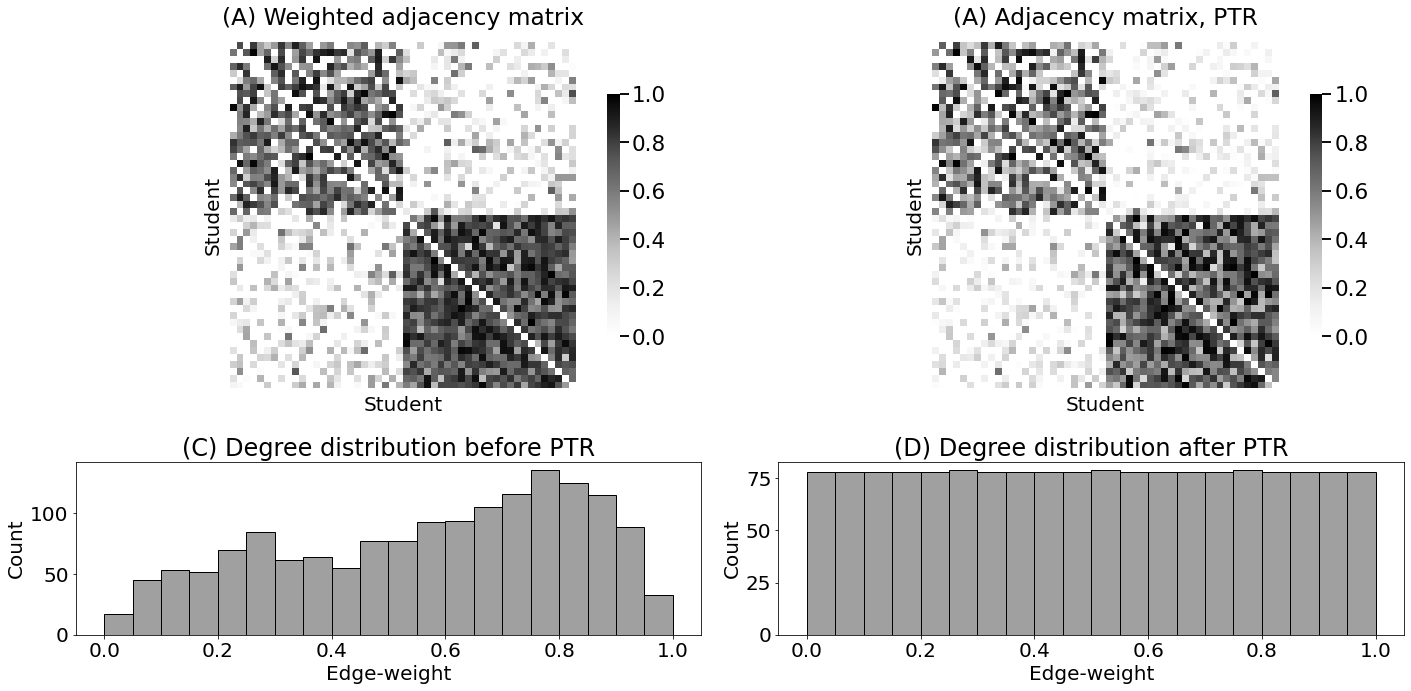
\includegraphics[width=\linewidth]{representations/ch4/Images/ptr.png}
    \caption[Passing to ranks to normalize edge-weights]{\textbf{(A)} the adjacency matrix before passing to ranks for the friendship network. \textbf{(B)} the adjacency matrix after passing to ranks. \textbf{(C)} the edge-weight histogram (including zero-weight edges) before passing to ranks. \textbf{(D)} the edge-weight histogram (including zero-weight edges) after passing to ranks.}
    \label{fig:ch4:ptr}
\end{figure}
The edge-weights for the adjacency matrix $R$ after \texttt{ptr} has the interpretation that each entry $r_{ij}$ which is non-zero is the \emph{quantile} of that entry amongst \emph{the other non-zero entries}. This is unique in that it is completely \emph{distribution-free}, which means that you don't need to assume anything about the distribution of the edge-weights to have an interpretable quantity. On the other hand, the $z$-score had the interpretation of the number of standard deviations from the mean, which is only a sensible quantity to compare if you assume the population of edge-weights are normally distributed.


Another useful quantity related to pass-to-ranks is known as the zero-boosted pass-to-ranks. Zero-boosted pass-to-ranks is conducted as in Algorithm \ref{alg:ch4:ptr_zb}.

\begin{algorithm}[h]
\SetAlgoLined
\caption{Zero-boosted pass to ranks}
    \KwData{$A$ is an adjacency matrix.}
    \KwResult{The adjacency matrix, after passing to ranks.}
    Identify all of the non-zero entries of the adjacency matrix $A$ and the zero-weighted entries of the adjacency matrix $A$.

    Let $n_{nz}$ be the number of non-zero entries of the adjacency matrix $A$, and $n_z$ be the number of zero-weighted entries of the adjacency matrix $A$. Note that $n_{nz} + n_z = n^2$, since $A$ has $n^2$ entries.

    Rank all of the non-zero edges in the adjacency matrix $A$, where for a non-zero entry $a_{ij}$, $rank(a_{ij}) = 1$ if $a_{ij}$ is the smallest non-zero edge-weight, and $rank(a_{ij}) = n_{nz}$ if $a_{ij}$ is the largest edge-weight. Ties are settled by using the average rank of the two entries.

    Report the weight of each non-zero entry $(i,j)$ as $r_{ij}' = \frac{n_z + rank(a_{ij})}{n^2 + 1}$, and for each zero entry as $r_{ij}' = 0$.
\end{algorithm}

The edge-weights for the adjacency matrix $R'$ after zero-boosted\texttt{ptr} have the interpretation that each entry $r_{ij}'$ is the quantile of that entry amongst \emph{all} of the entries. Let's instead use zero-boosted\texttt{ptr} on your network:

\begin{lstlisting}[style=python]
RA_friend_zb = pass_to_ranks(A_friend, method="zero-boost")
\end{lstlisting}
We show the adjacency matrix after zero-boosted \texttt{ptr}, along with the edge-weight histogram (including zero-weight edges), in Figure \ref{fig:ch4:ptr_zb}.

\begin{figure}[h]
    \centering
    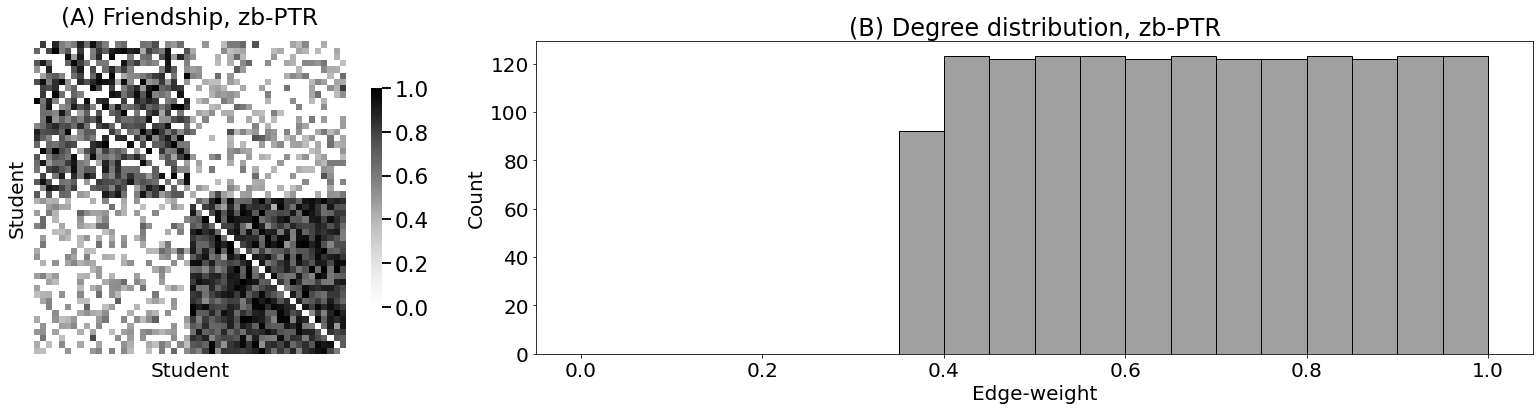
\includegraphics[width=\linewidth]{representations/ch4/Images/ptr_zb.png}
    \caption[Zero-Boosted PTR]{\textbf{(A)} the adjacency matrix, after zero-boosted\texttt{ptr}. \textbf{(B)} the edge-weight histogram, after zero-boosted\texttt{ptr}. Compare this to Figure \ref{fig:ch4:ptr}(B) and \ref{fig:ch4:ptr}(D), respectively.}
    \label{fig:ch4:ptr_zb}
\end{figure}

\paragraph{Thresholding as a decimation of ranking}
As it turns out, the thresholding approach you learned in Section \ref{sec:ch4:regularization:thresholding} can be thought of as a \emph{decimation} of ranking, assuming that the ranking implementation handles ties randomly (the implementation in\texttt{graspologic} does not, as ties are settled by the average rank, but we would encourage you to implement one that \emph{does} as an exercise). For instance, if you picked a threshold of $0.5$, there is some corresponding rank (or value in between two ranks), where all of the elements of the adjacency matrix with a rank lower than a given threshold $\tau_r$ have corresponding weights lower than $\tau$ and all of the elements of the adjacency matrix with a rank higher than a given threshold $\tau_r$ have corresponding weights higher than $\tau$. Then, you can simply threshold the ranked adjacency matrix using $\tau_r$.

\paragraph{Logging reduces magnitudinal differences between edges}
\label{sec:ch4:regularization:logscale}

When we look at the distribution of non-zero edge-weights for the activity/hobby network or the friendship network, we notice a strange pattern, known as a \emph{right-skew}. This is shown in Figure \ref{fig:ch4:log}(A). Informally, a distribution is \emph{right-skewed} if a large fraction of the points take relatively small values, and then a small portion of the points take relatively large values. Notice in this figure, for instance, that most points have an edge weight between $0$ and $2$, but and a small portion of points have an edge-weight between $2$ and $10$. This is called a ``right-skew'' because the histogram ``tails off'' as the values go to the right (increase). 


What if you want to make these large values more similar in relation to the smaller values, but you simultaneously want to preserve properties of the underlying distribution of the edge-weights? Well, you can't use\texttt{ptr`, because `ptr} will throw away all of the information about the edge-weight distribution other than the ordinal relationship between pairs of edges. To interpret what this means, you might think that there is a big difference between sharing no interests compared to three interests in common, but there is not as much of a difference in sharing ten interests compared to thirteen interests in common.

To do this, we instead turn to the logarithm function. The logarithm function $log_{10}(x)$ is defined for positive values $x$ as the value $c_x$ where $x = 10^{c_x}$. In this sense, it is the "number of powers of ten" to obtain the value $x$. The logarithm function is shown in Figure \ref{fig:ch4:log}(B).

\begin{figure}
    \centering
    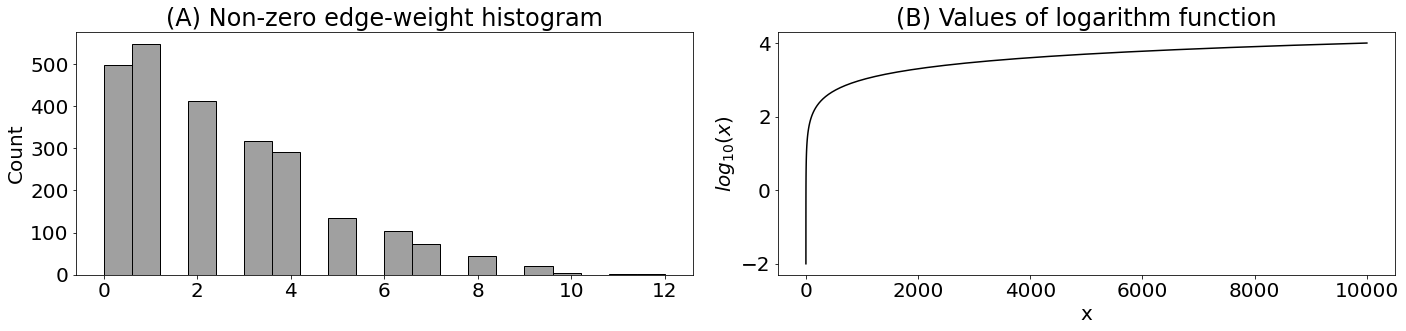
\includegraphics[width=\linewidth]{representations/ch4/Images/log.png}
    \caption[Heavy tailed edge-weights]{\textbf{(A)} The non-zero edge-weight histogram for the activity/hobby network. Notice that the histogram ``tails off'' towards the right. \textbf{(B)} The value for the base-$10$ logarithm function for given values of $x$.}
    \label{fig:ch4:log}
\end{figure}

What is key to noice about this function is that, as $x$ increases, the log of $x$ increases by a \emph{decreasing} amount. Let's imagine you have three values, $x = .001$, $y = .1$, and $z = 10$. A calculator will give you that $log_{10}(x) = -3, log_{10}(y) = -1$, and $log_{10}(z) = 1$. Even though $y$ is only $.099$ units bigger than $x$, its logarithm $log_{10}(y)$ exceeds $log_{10}(x)$ by two units. on the other hand, $z$ is $9.9$ units bigger than $y$, but yet its logarithm $log_{10}(z)$ is still the same two units bigger than $log_{10}(y)$. This is because the logarithm is instead looking at the fact that $z$ is \emph{one} power of ten, $y$ is $-1$ powers of ten, and $z$ is $-3$ powers of ten. The logarithm has \emph{collapsed} the huge size difference between $z$ and the other two values $x$ and $y$ by using exponentiation with \emph{base} ten. 


In this sense, you can also use the logarithm function for your network to reduce the huge size difference between the values in your activity/hobby network. However, we must first add a slight twist: to do this properly and yield an interpretable adjacency matrix, you need to \emph{augment} the entries of the adjacency matrix \emph{if} it contains zeros. This is because the $log_{10}(0)$ is \emph{not defined}. To augment the adjacency matrix, we'll basically ``inflate'' these values by a magnitude that is negligibly small. We show how to implement this in Algorithm \ref{alg:ch4:log_xfm}.

\begin{algorithm}[h]
    \SetAlgoLined
    \caption{Log transforming a network with zero-weight edges.}
    \KwData{$A$ is an adjacency matrix. \newline $b$ the base to log transform with.}
    \KwResult{The adjacency matrix, after log transformation.}

    Identify the entries of $A$ which take a value of zero.

    Identify the smallest entry of $A$ which is not-zero, and call it $a_m$.

    Compute a value $\epsilon$ which is an \emph{order of magnitude} smaller than $a_m$. Since you are taking powers of $b$, a single order of magnitude would give us that $\epsilon = \frac{a_m}{b}$. 

    Take the augmented adjacency matrix $A'$ to be defined with entries $a_{ij}' = a_{ij} + \epsilon$.

    Log transform $A'$ with a base of $b$.
\end{algorithm}

The first process of this procedure is called a \emph{zero augmentation}. We can code up the log transformation as follows:


\begin{lstlisting}[style=python]
def augment_zeros(X, base=10):
    if np.any(X < 0):
        raise TypeError("The logarithm is not defined for negative values!")
    am = np.min(X[np.where(X > 0)])  # the smallest non-zero entry of X
    eps = am/base  # epsilon is one order of magnitude smaller than the smallest non-zero entry
    return X + eps  # augment all entries of X by epsilon
def log_transform(X, base=10):
    """
    A function to log transform an adjacency matrix X, which may
    have zero-weight edges.
    """
    X_aug = augment_zeros(X, base=base)
    return np.log(X_aug)/np.log(base)

A_activity_log = log_transform(A_activity)
\end{lstlisting}

We plot the untransformed and log-transformed activity/hobby network in Figure \ref{fig:ch4:log_xfm}. 

When you plot the augmented and log-transformed data, what you see is that many of the edge-weights you originally might have thought were zero if you only looked at a plot were, in actuality, \emph{not} zero. In this sense, for non-negative weighted networks, log transforming after zero-augmentation is often very useful for visualization to get a sense of the magnitudinal differences that might be present between edges, since you can get a better feel for how different the big weights are from the smaller weights.

\begin{figure}[h]
    \centering
    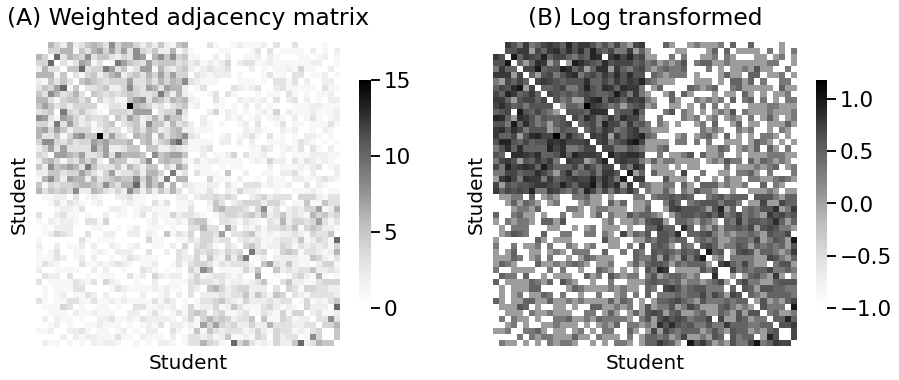
\includegraphics[width=\linewidth]{representations/ch4/Images/log_xfm.png}
    \caption[Log-transforming heavy-tailed edge-weights]{\textbf{(A)} The weighted adjacency matrix for the activity/hobby network. Notice that there are many entries which are very small, and it is hard to discern which entries are zero from the entries that are just tiny. \textbf{(B)} The activity/hobby network, after log transformation. Notice that the edges which are zero are readily apparent in the plot, and we have a better sense of the range of non-zero elements visually as well (they tend to fall between $0$ and $1$, so are different by approximately a power of $10$).}
    \label{fig:ch4:log_xfm}
\end{figure}
